\section{Measuring reactive components} \label{sec:MeasureReactiveComponents}
When no impedance analyzer is available, impedance can still be estimated by means of other methods, one such method will be introduced here.

Impedance is the magnitude and phase angle between voltage and current, and thus to measure impedance, both voltage and current must be measured together with
their phase difference. From this it follows that to characterize the impedance of a device, voltage, current and their phase must be measured. An LCR meter measures exactly these parameters
at the desired test frequency, LCR meters, unlike oscilloscopes and signal generators, are however not a common laboratory instrument. The authors of this document are both
electronics technicians and testify to the quote from Tektronix \Cite{TextronixZMeas} "\textit{It is not always easy to find an LCR meter}". 

To measure the impedance of a component, an oscilloscope, signal generator and precision resistor can however be used as an alternative to an LCR meter. Such a setup is illustrated in figure \ref{fig_2.1_ImpedanceMeas}, where a signal generator is used to excite the unknown device, and a reference resistor is used as a shunt to measure the current. An oscilloscope is then used to measure both the amplitude and phase of voltage and current. 

\begin{figure}[H]
    \centering
    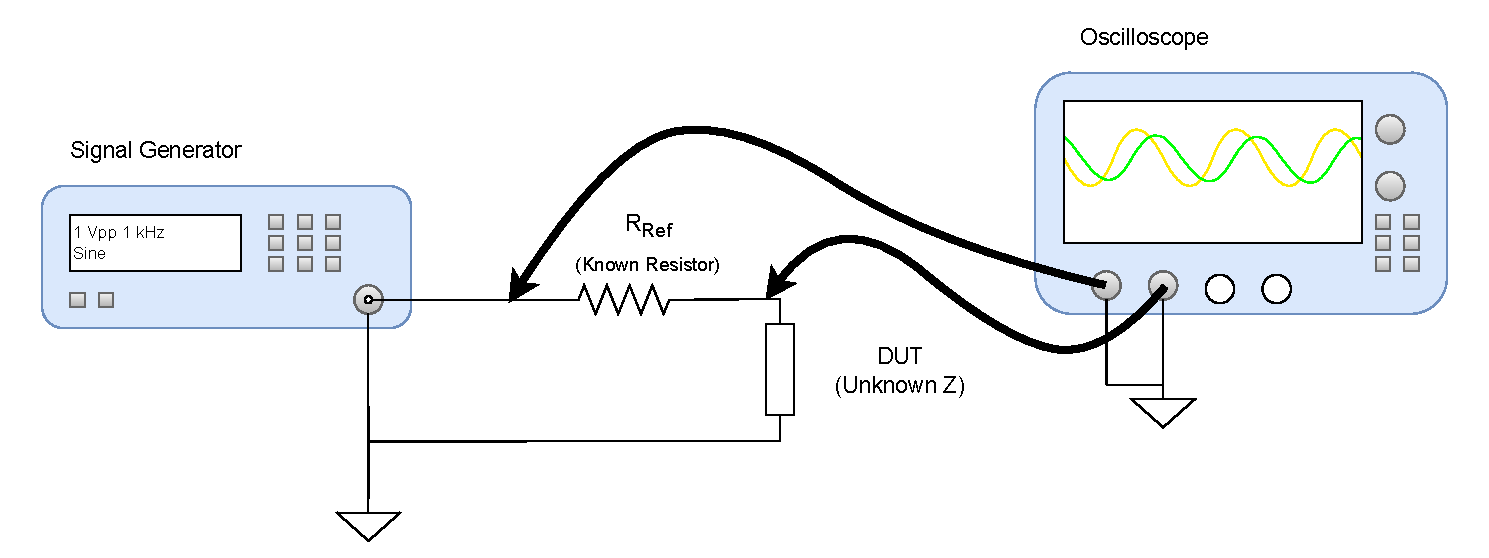
\includegraphics[width=1\textwidth]{Sections/2_ProblemAnalysis/Figures/ScopeGenZMeas.pdf}
    \caption{Impedance measurement with an oscilloscope and signal generator.}
    \label{fig_2.1_ImpedanceMeas}
\end{figure}

The methods shown in figure \ref{fig_2.1_ImpedanceMeas} is also described in the application note \textit{"Capacitance and Inductance Measurements Using an oscilloscope and a Function Generator"} from Tektronix \Cite{TextronixZMeas}. This application note also indicates that the accuracy of such a setup is rather limited.

Not only is this method limited by its accuracy, it is also limited with regards to impedance and frequency range. At higher frequencies parasitic elements such as the oscilloscope probe input capacitance, will influence the measurement accuracy. The range of the system is also limited by the input impedance of the probes and the reference resistor. If very large impedances are to be measured, the input impedance of the oscilloscope will influence the measurement. Generally, the range resistor will need to be kept around  the same value as the magnitude of the measured impedance. This results in a small reference resistor for smaller impedances, and thus in order to generate a measurable voltage drop across the resistor, a rather large current might be required. All of these elements limits the effectiveness of this method, and makes it rather time consuming, not to mentioned the numerous areas where errors can be introduced.
